% Nexus Terminal — User Guide. Build: make (in docs/guide), or: lualatex nexus-guide && lualatex nexus-guide
\documentclass[10pt,twoside,openany]{book}
\usepackage{nexus-guide}

\hypersetup{pdftitle={Nexus Terminal: The User Guide}, pdfauthor={Andy Dixon},
  pdfsubject={SSH, Telnet, RAW, Serial, VNC, IRC and GitHub in one native app}}

\begin{document}
\frontmatter
\pagestyle{empty}

% --- Cover ------------------------------------------------------------------------------
\pagecanvas{
  \fill[ink] (pg.south west) rectangle (pg.north east);
  \shade[left color=accent, right color=violet, opacity=0.55]
    ([yshift=-60mm]pg.north west) -- ([yshift=-20mm]pg.north east) --
    ([yshift=-130mm]pg.north east) -- ([yshift=-170mm]pg.north west) -- cycle;
  \shade[left color=teal, right color=accent, opacity=0.35]
    ([yshift=-150mm]pg.north west) -- ([yshift=-120mm]pg.north east) --
    ([yshift=-150mm]pg.north east) -- ([yshift=-185mm]pg.north west) -- cycle;
  \node[anchor=north east, inner sep=0pt] at ([xshift=-22mm, yshift=-24mm]pg.north east)
    {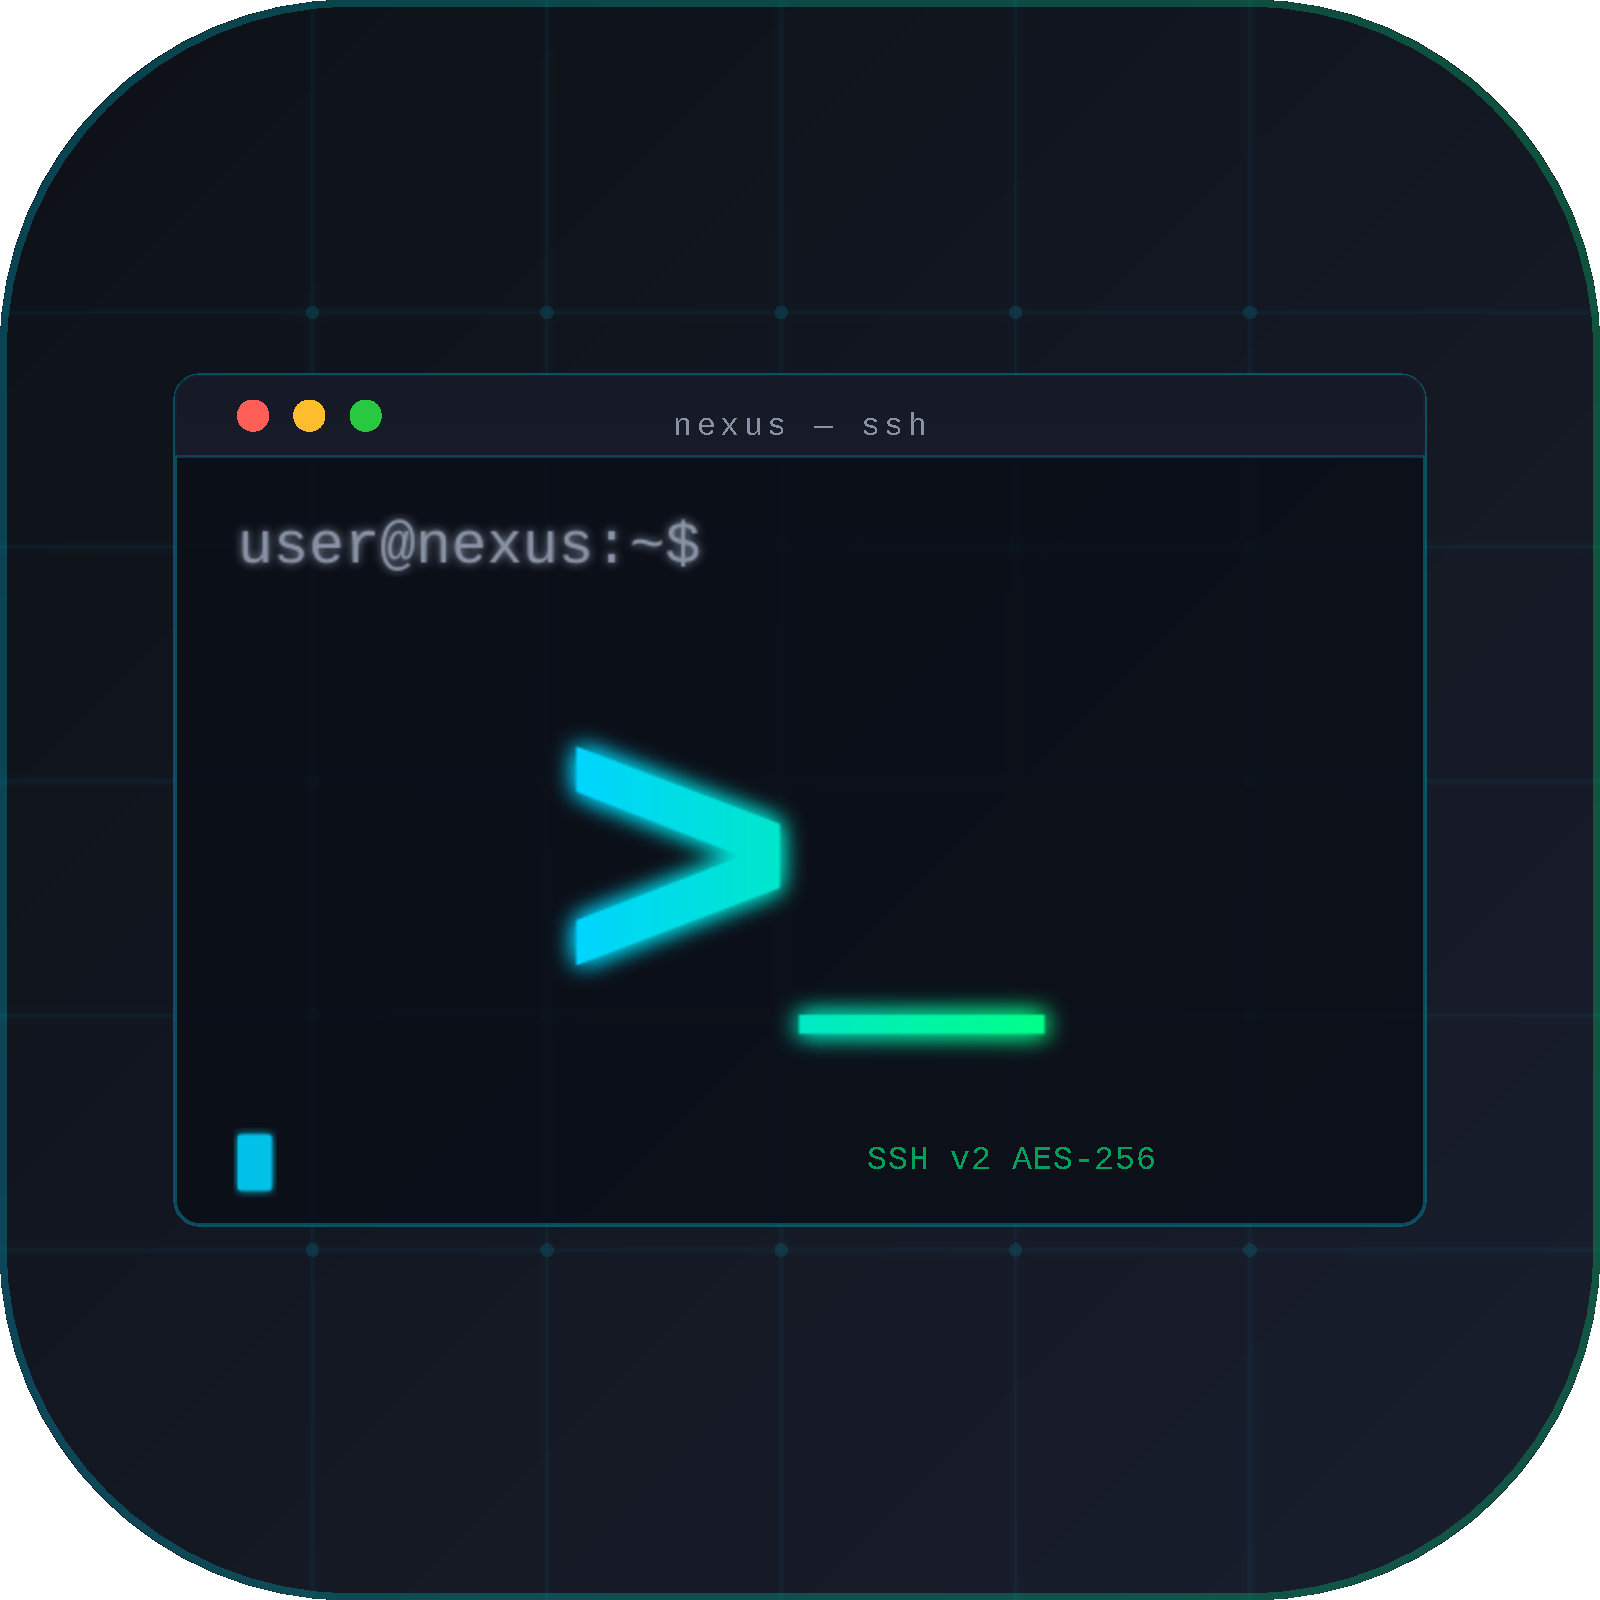
\includegraphics[width=34mm]{img/logo.pdf}};
  \node[anchor=north west, text=white!70!ink, font=\heavy\small] at ([xshift=22mm, yshift=-30mm]pg.north west)
    {THE USER GUIDE};
  \node[anchor=north west, text=white, font=\heavy\fontsize{58}{60}\selectfont, text width=170mm]
    at ([xshift=22mm, yshift=-36mm]pg.north west) {Nexus\\[-2pt]Terminal};
  \node[anchor=north west, text=white, font=\Large, text width=150mm]
    at ([xshift=22mm, yshift=-88mm]pg.north west)
    {Every terminal you need. One window.\\Zero faff.};
  \node[anchor=north west, text=white!65!ink, font=\normalsize, text width=150mm]
    at ([xshift=22mm, yshift=-110mm]pg.north west)
    {SSH\enspace·\enspace Telnet\enspace·\enspace RAW TCP\enspace·\enspace Serial\enspace·\enspace VNC\enspace·\enspace IRC\enspace·\enspace GitHub\enspace·\enspace Local shells};
  \node[anchor=south west, inner sep=0pt] at ([xshift=22mm, yshift=22mm]pg.south west)
    {\begin{tikzpicture}
      \node[inner sep=0pt, draw=white!25!ink, line width=0.6pt, rounded corners=4pt] {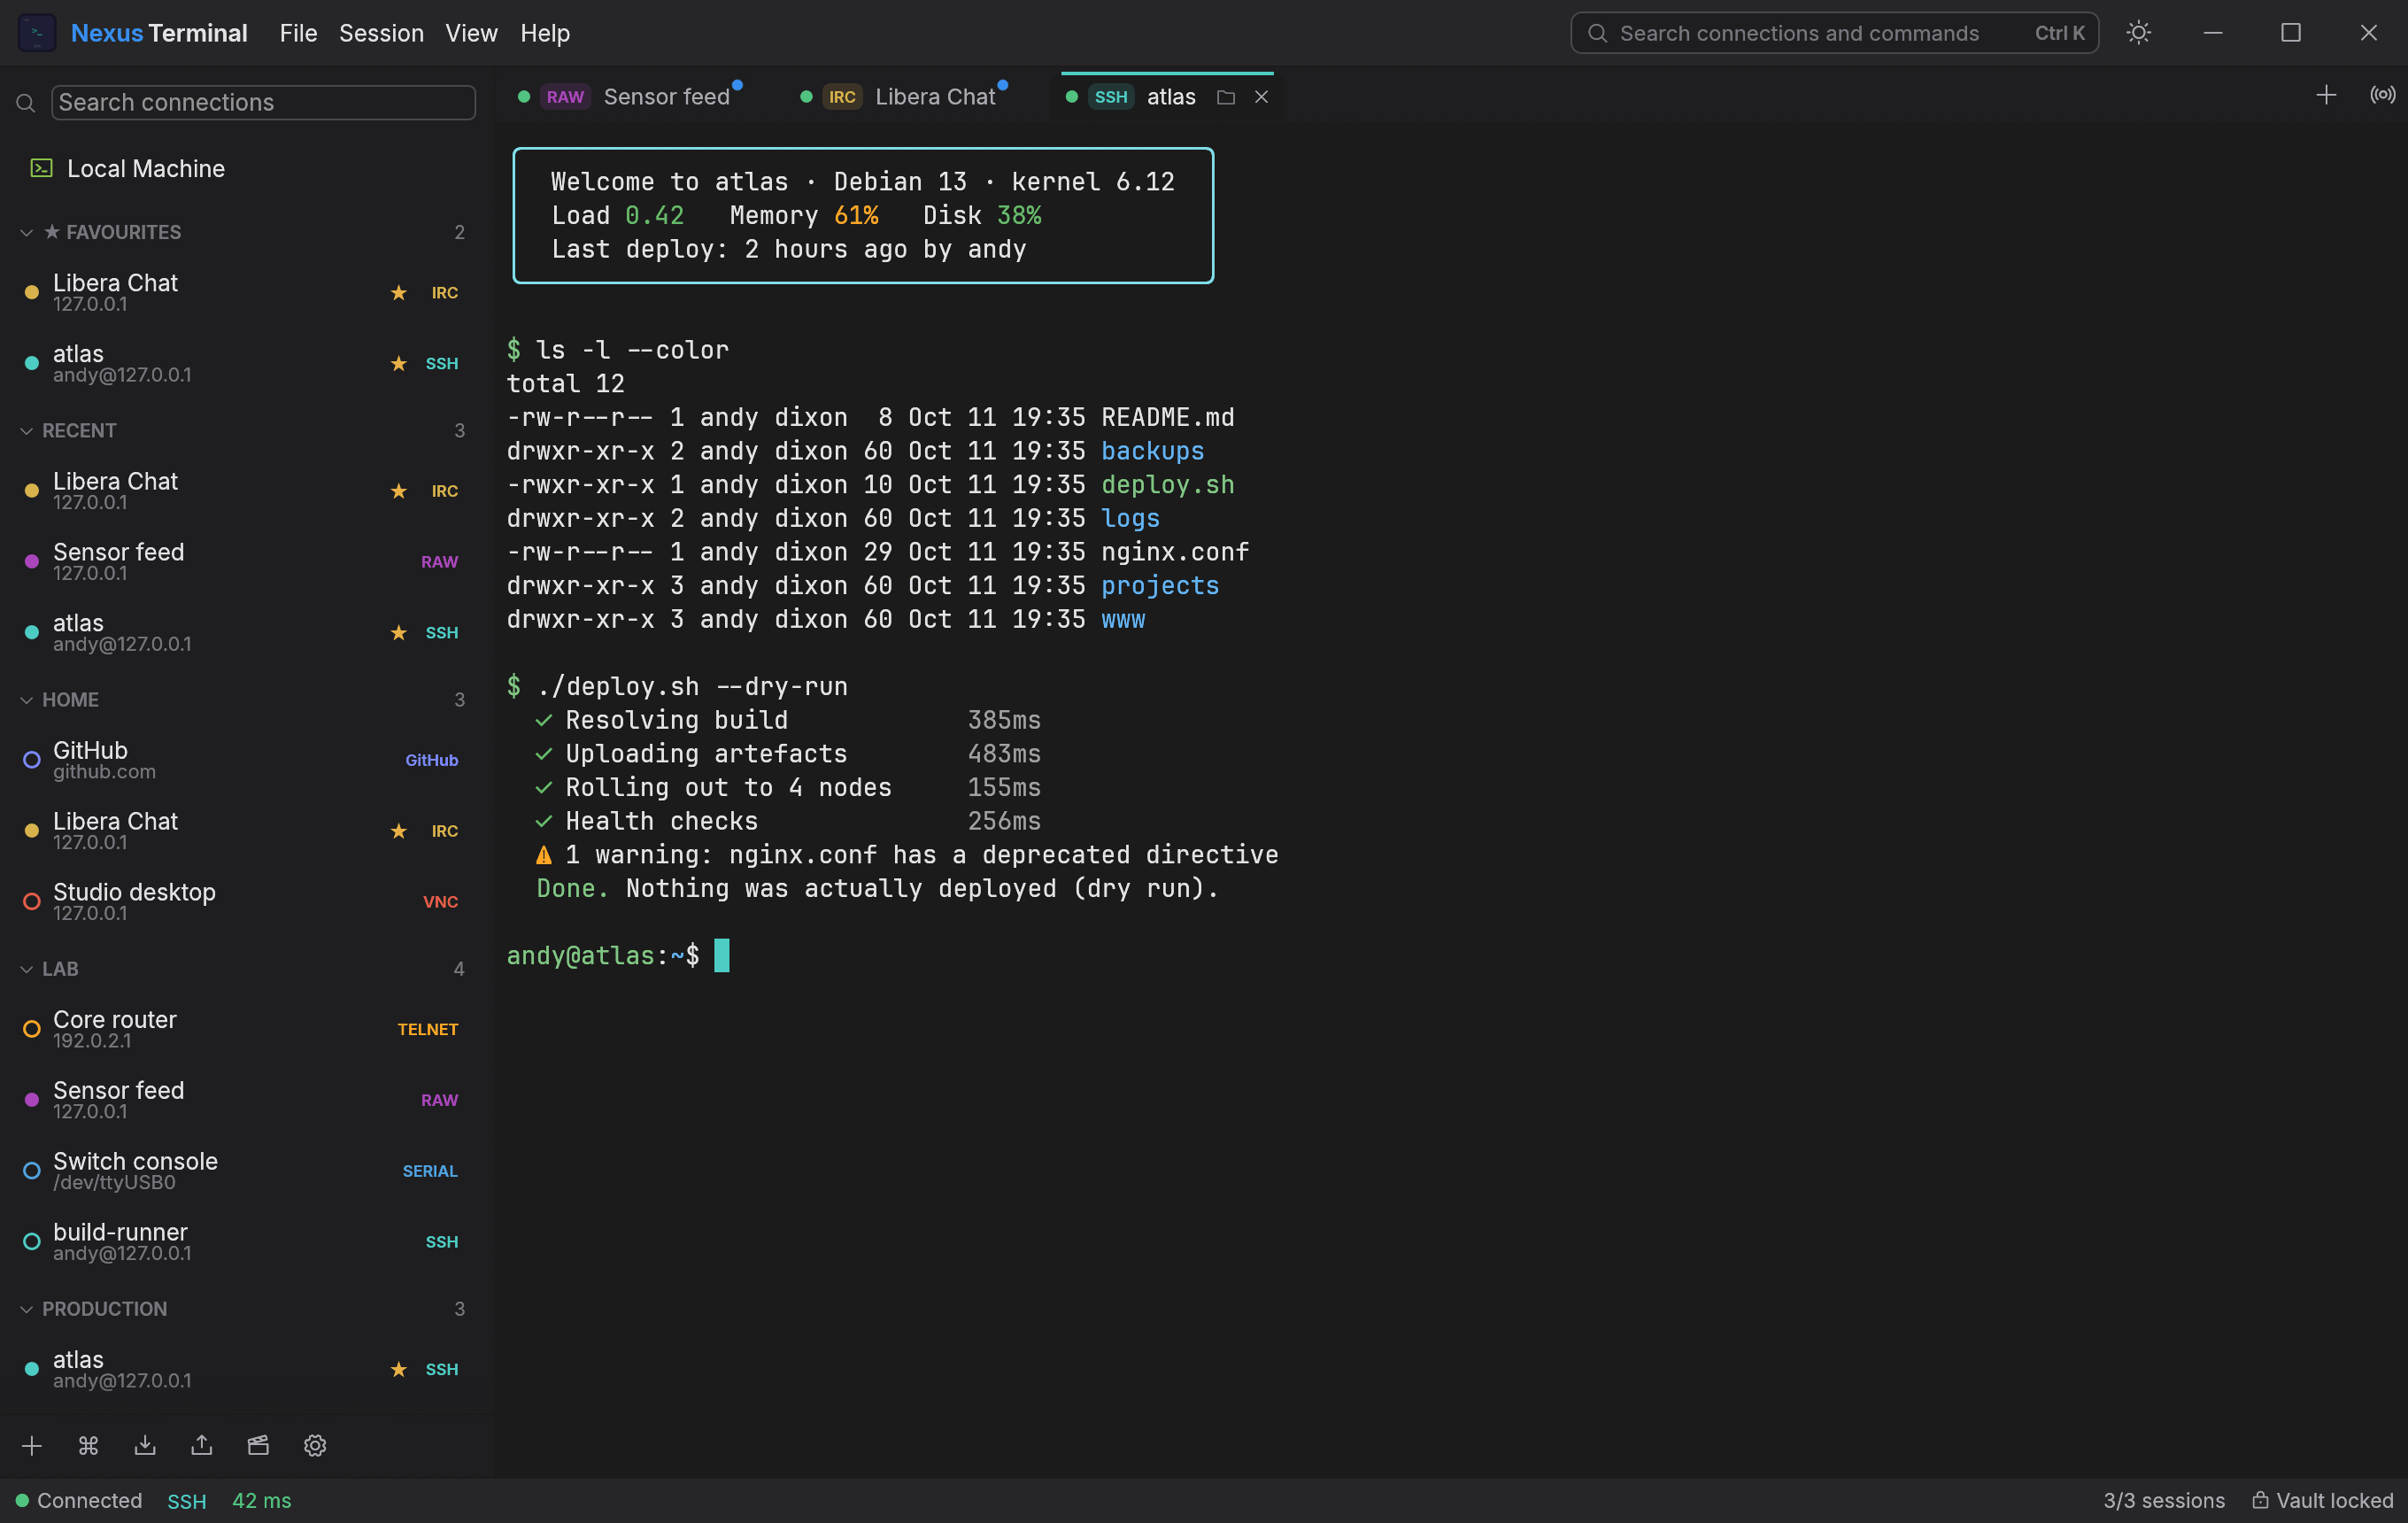
\includegraphics[width=166mm]{img/ssh.png}};
    \end{tikzpicture}};
  \node[anchor=south east, text=white!55!ink, font=\footnotesize, align=right]
    at ([xshift=-22mm, yshift=24mm]pg.south east) {Version 0.1\\October 2026\\dixon.cx};
}\null
\cleardoublepage

% --- How to use this guide ----------------------------------------------------------------
\colorlet{partcol}{accent}
{\heavy\fontsize{30}{34}\selectfont\color{ink} Start here.\par}
\vspace{2pt}{\large\color{muted} (Yes, even if you never read manuals. \emph{Especially} then.)\par}
\vspace{10pt}

This guide is built for skimming. You do \textbf{not} have to read it in order, cover to cover, like it's
homework. Find the bit you need, grab it, get back to work. Every chapter opens with the time it takes and
what you'll be able to do afterwards, and a \textbf{TL;DR} if you only want the gist.

\vspace{4pt}
{\heavy\large\color{ink}\iMap\enspace I just want to…}\par\vspace{2pt}
\renewcommand\arraystretch{1.5}
\begin{tabularx}{\linewidth}{@{}X>{\raggedleft\arraybackslash}p{52mm}@{}}
  \toprule
  …get connected to something \emph{right now} & \hyperref[ch:start]{Five-minute start}, p.\,\pageref{ch:start}\\
  …work out what all the buttons do & \hyperref[ch:tour]{The grand tour}, p.\,\pageref{ch:tour}\\
  …SSH into a server (keys, jump hosts, 2FA) & \hyperref[ch:ssh]{SSH}, p.\,\pageref{ch:ssh}\\
  …talk to a router or Arduino over a USB cable & \hyperref[ch:serial]{Serial}, p.\,\pageref{ch:serial}\\
  …copy files to and from a server & \hyperref[ch:files]{Files}, p.\,\pageref{ch:files}\\
  …type the same thing into ten servers at once & \hyperref[ch:repeat]{Never type it twice}, p.\,\pageref{ch:repeat}\\
  …keep my passwords safe & \hyperref[ch:secrets]{Passwords \& the vault}, p.\,\pageref{ch:secrets}\\
  …move over from Alchementary Link & \hyperref[ch:move]{Moving house}, p.\,\pageref{ch:move}\\
  …fix something that's broken & \hyperref[part:fix]{When things go wrong}, p.\,\pageref{ch:trouble}\\
  …just see the keyboard shortcuts & \hyperref[app:keys]{The cheat sheet}, p.\,\pageref{app:keys}\\
  \bottomrule
\end{tabularx}

\vspace{8pt}
{\heavy\large\color{ink}\iSparkle\enspace The little boxes}\par\vspace{-2pt}
\begin{multicols}{2}\small
\begin{tldr}The whole chapter in three lines.\end{tldr}
\begin{quickwin}Something you can try in under a minute.\end{quickwin}
\begin{protip}A trick that saves you time later.\end{protip}
\columnbreak
\begin{headsup}A thing that might trip you up.\end{headsup}
\begin{danger}Could lose data or weaken security. Read it.\end{danger}
\begin{sidequest}Interesting, but not needed to get the job done.\end{sidequest}
\end{multicols}

\vspace{-6pt}
{\small\color{muted}\textbf{Shortcuts:} \mod{} means \kbd{Ctrl} on Windows and Linux, \kbd{\ph{E1C4}} (Command) on a Mac. So
\keys{\mod+K} is \kbd{Ctrl}+\kbd{K} or \kbd{\ph{E1C4}}+\kbd{K} depending on your machine.}

\clearpage
\pagestyle{plain}
{\hypersetup{linkcolor=body}\tableofcontents}
\clearpage

\mainmatter
\pagestyle{fancy}
\guidepart{accent}{Get going}{Get going}
  {From zero to connected before your tea goes cold.}
  {\partitem{\iRocket}{Five-minute start}
   \partitem{\iMap}{The grand tour}
   \partitem{\iList}{Profiles: your address book}}

% =========================================================================================
\chapter{Five-minute start}\label{ch:start}
\chapmeta{5 minutes}{You'll be connected to something and know the one shortcut that matters}

\begin{tldr}
Install it, open it, press \keys{\mod+N}, fill in a host, hit \ui{Create \& Connect}. Done.
Lost? Press \keys{\mod+K} and type what you want.
\end{tldr}

\section{Install it}

Grab the zip for your machine from \code{dixon.cx/downloads/nexus}. They're named
\code{NexusTerminal-<os>-<arch>.zip}, so a modern Mac wants \code{darwin-arm64} and most PCs want \code{amd64}.

\begin{description}
  \item[\iDesktop\enspace Windows] Unzip it and run \code{NexusTerminal-windows-amd64.exe}. No installer, no admin rights,
    nothing in the registry. Pop it somewhere sensible like \code{C:\textbackslash Tools} and pin it to the taskbar.
  \item[\iDesktop\enspace macOS] Unzip it and drag \code{NexusTerminal-darwin-arm64.app} into \ui{Applications}. If macOS
    grumbles that it can't check the developer, right-click the app, choose \ui{Open}, then \ui{Open} again. You only
    have to do that once.
  \item[\iDesktop\enspace Linux] Unzip it and run \code{./install.sh}. It copies \code{nexus-terminal} into
    \code{~/.local/bin} and adds a launcher entry with the icon, so it turns up in your app menu.
    (Make sure \code{~/.local/bin} is on your \code{PATH}.)
\end{description}

\begin{sidequest}[Build it yourself]
It's a single Rust program. With Rust installed: \code{cd rust \&\& cargo run --release}. The finished binary lands in
\code{rust/target/release/nexus-terminal}. The build guide in \code{docs/build-and-release.md} has the full story.
\end{sidequest}

\section{Open it}

The first time you open Nexus Terminal you get a calm, empty welcome screen. Three buttons, four shortcuts. That's it.

\shot{welcome.png}{The welcome screen. Your saved connections will live down the left; here there are a few already.}

\begin{headsup}[Got more than one computer?]
Point \ui{Profile sync} at a shared folder and your connections follow you around. See
\hyperref[ch:move]{Moving house} on p.\,\pageref{ch:move}.
\end{headsup}

\section{Make your first connection}

\begin{enumerate}
  \item Click \ui{New Connection}, or press \keys{\mod+N}.
  \item Pick the protocol along the top: \proto[teal]{SSH}, \proto[amber]{Telnet}, \proto[violet]{RAW TCP},
        \proto[slate]{GitHub}, \proto[rose]{VNC}, \proto[rose]{RDP}, \proto[amber]{IRC} or \proto[accent]{Serial}.
  \item Fill in the \ui{General} bit: a \ui{Display Name} you'll recognise, the \ui{Host}, the \ui{Port}
        and your \ui{Username}.
  \item Click \ui{Create \& Connect}.
\end{enumerate}

That's genuinely it. A tab opens, you log in, and next time it's one click in the sidebar.

\crop{editor-new.png}{1515}{40}{0}{70}{0.52\linewidth}{A brand-new SSH profile. Only the top few fields are needed to get going.}

\begin{quickwin}
Click \ui{Test} before you save. Nexus Terminal checks the host and port are reachable and tells you the
round-trip time. If that fails, no amount of password-fiddling will help, so it's a great first check.
\end{quickwin}

\section{Two shortcuts for impatient people}

\subsection{Quick Connect}
Press \keys{\mod+Shift+Q}.
For a one-off session you don't want to save. Pick SSH, Telnet, RAW, IRC or Serial, type the host (or serial
device), hit \kbd{Enter}. Nothing gets saved.

\crop{quick.png}{951}{620}{946}{481}{0.5\linewidth}{Quick Connect. In, out, nobody gets hurt.}

\subsection{Local terminal}
Click \ui{Local Machine} at the top of the sidebar (or \ui{Local} on the welcome screen) for a shell on
\emph{this} computer. When you type \code{exit}, the tab says \code{[Exited - press enter to restart]}.
Press \kbd{Enter} and you've got a fresh shell in the same tab.

\section{The one shortcut to rule them all}

\begin{center}
\begin{tcolorbox}[enhanced, width=0.8\linewidth, arc=10pt, boxrule=0pt, colback=ink, fontupper=\color{white},
  halign=center, top=10pt, bottom=10pt, drop fuzzy shadow]
{\scalebox{2.4}{\keys{\mod+K}}}\par\vspace{6pt}\par\vspace{4pt}
{\color{white!70!ink} The command palette. If you remember nothing else, remember this.}
\end{tcolorbox}
\end{center}

Type a few letters of \emph{anything}: a connection name, a tab, ``theme'', ``split'', ``lock'', ``snippets''. Use
\kbd{↑}\kbd{↓} to pick, \kbd{Enter} to go, \kbd{Esc} to bail. It's fuzzy, so ``atl'' finds \emph{atlas} and
``sft'' finds the \emph{SFTP Browser}.

\crop{palette.png}{755}{732}{733}{154}{0.72\linewidth}{The command palette: every connection, tab and action in one searchable list.}

\begin{quickwin}[Your five-minute checklist]
\begin{checklist}
  \item Installed and opened Nexus Terminal
  \item Opened a \ui{Local Machine} tab and typed \code{exit}, then \kbd{Enter} to get it back
  \item Made a profile with \keys{\mod+N} and clicked \ui{Test}
  \item Connected to it
  \item Opened the palette with \keys{\mod+K} and found something by typing three letters
\end{checklist}
All ticked? You're officially more productive than you were five minutes ago. \iConfetti
\end{quickwin}

% =========================================================================================
\chapter{The grand tour}\label{ch:tour}
\chapmeta{4 minutes}{You'll know what every bit of the window is for}

\begin{tldr}
Connections on the left. Sessions in tabs across the top. The terminal in the middle. Status along the bottom.
Everything else is one \keys{\mod+K} away.
\end{tldr}

\begin{annotated}{ssh.png}
  \callout{1}{0.124}{0.022}
  \callout{2}{0.66}{0.022}
  \callout{3}{0.888}{0.022}
  \callout{4}{0.22}{0.067}
  \callout{5}{0.03}{0.152}
  \callout{6}{0.53}{0.063}
  \callout{7}{0.966}{0.063}
  \callout{8}{0.62}{0.42}
  \callout{9}{0.16}{0.945}
  \callout{10}{0.26}{0.985}
  \callout{11}{0.86}{0.985}
\end{annotated}

\begin{multicols}{2}\small
\begin{description}[leftmargin=0pt, labelsep=0.4em]
  \item[\num{1} Menus] \menu{File}, \menu{Session}, \menu{View} and \menu{Help}. Drag the title bar to move the
        window; double-click it to maximise.
  \item[\num{2} Palette] The search box is the command palette. Click it or press \keys{\mod+K}.
  \item[\num{3} Light/dark] Flip between the dark and light themes in one click.
  \item[\num{4} Search] Fuzzy-search your connections by name, host, tag or protocol.
  \item[\num{5} Sections] \ui{Local Machine}, \ui{Favourites} \iStar, \ui{Recent} (your last five), then one section
        per group. Click a header to fold it away.
  \item[\num{6} Tabs] One per session, with a coloured state dot, protocol badge and close button. SSH tabs get a
        little \iFolder{} for files. A blue dot means ``new output while you weren't looking''.
  \item[\num{7} New \& broadcast] \ui{+} opens a new connection; \iBroadcast{} toggles broadcast mode.
  \item[\num{8} Workspace] Your terminal (or IRC chat, VNC desktop, GitHub list…). Split it into panes, too.
  \item[\num{9} Footer] New connection, palette, import, export, recordings and settings.
  \item[\num{10} Status] State, protocol and live latency for SSH. Shows \ui{REC} while recording and
        \ui{BROADCAST} when broadcasting.
  \item[\num{11} Sessions \& vault] How many sessions are connected and whether the vault is locked. Click the vault to
        open security settings.
\end{description}
\end{multicols}

\begin{protip}
Drag the right-hand edge of the sidebar to make it wider or narrower. Toasts (the little pop-up messages in the
top-right) tidy themselves away after a few seconds; click \ui{×} if you're impatient.
\end{protip}

\section{Three looks}

Nexus Terminal comes in \ui{Pro} (the default, a soft charcoal), \ui{Midnight} (darker, bluer, for 2\,a.m.
deploys) and \ui{Light} (for sunny days and projectors). Switch with the \iBulb{} button in the title bar, the
\menu{View} menu, or type ``theme'' into the palette.

\shotpair{welcome-midnight.png}{Midnight}{ssh-light.png}{Light, with a session open}

The \emph{terminal} has its own colour schemes too: eleven of them, including \ui{Dracula}, \ui{Nord},
\ui{Tokyo Night}, \ui{Catppuccin Mocha} and \ui{Rosé Pine}. Those live in \menu{Settings\then Terminal} and the \menu{View} menu.

% =========================================================================================
\chapter{Profiles: your address book}\label{ch:profiles}
\chapmeta{6 minutes}{You'll keep dozens of connections tidy without thinking about it}

\begin{tldr}
A \emph{profile} is a saved connection. Give it a name and a group, star the ones you use daily, and
right-click for everything else. Ctrl-click to select lots at once.
\end{tldr}

\section{Create, edit, copy}

\begin{itemize}
  \item \textbf{New:} \ui{+} in the sidebar footer or tab strip, \keys{\mod+N}, or right-click a group header and choose
        \ui{New connection in …} (it lands in that group automatically).
  \item \textbf{Edit:} double-click a profile, or right-click\then\ui{Edit}. The editor slides in on the right.
  \item \textbf{Copy:} right-click\then\ui{Duplicate}. Great for ``same as web-01 but web-02''.
  \item \textbf{Delete:} right-click\then\ui{Delete}. This also deletes the saved passwords for that profile.
\end{itemize}

\crop{editor-ssh.png}{1515}{40}{0}{70}{0.52\linewidth}{Editing an existing SSH profile. The editor scrolls; sections are grouped so you can ignore most of them.}

\subsection{What goes in a profile}

Every profile has the same \ui{General} section, then sections specific to its protocol (Part 2 covers each
one). The common bits are:

\renewcommand\arraystretch{1.4}
\begin{tabularx}{\linewidth}{@{}>{\leavevmode\heavy\color{ink}}p{32mm}X@{}}
  \toprule
  Display Name & What you'll see in the sidebar. Make it obvious: ``db-primary'', not ``server 3''.\\
  Host / Port  & Where to connect. Serial profiles have a \ui{Device} instead.\\
  Group        & Pick an existing group or type a new name to create one.\\
  Description  & One line shown on hover.\\
  Terminal     & Font, size (8–36), scrollback (0–100\,000 lines) and cursor style, just for this profile.\\
  Tags \& Notes & Comma-separated tags (searchable!) and free-form notes for future-you.\\
  \bottomrule
\end{tabularx}

Each protocol adds its own sections underneath. Here are four of them side by side; Part~2 goes through each one.

\begin{center}
\newcommand\mini[2]{\begin{minipage}[t]{0.24\linewidth}\centering\includegraphics[width=\linewidth, trim=1515 600 0 70, clip]{img/#1}\par\vspace{2pt}{\scriptsize\color{muted}#2}\end{minipage}}
\mini{editor-telnet.png}{Telnet}\hfill\mini{editor-raw.png}{RAW TCP}\hfill\mini{editor-vnc.png}{VNC}\hfill\mini{editor-irc.png}{IRC}
\end{center}

\begin{protip}[Tags are secretly brilliant]
Tag things by where they live and what they do (\code{eu-west}, \code{db}, \code{customer-x}). The sidebar search
matches tags, so typing ``db'' instantly narrows hundreds of profiles to the database servers.
\end{protip}

\section{Favourites, groups and Recent}

\begin{itemize}
  \item Right-click\then\ui{Add to Favourites} pins a profile into the \ui{\iStar\ Favourites} section at the top.
  \item \ui{Recent} always shows the last five things you connected to. You don't have to do anything.
  \item Groups are just the \ui{Group} field. No group? It goes in \ui{Ungrouped}.
\end{itemize}

\section{Do lots at once}

Hold \kbd{Ctrl} (\kbd{\ph{E1C4}} on a Mac) and click several profiles. A bar appears at the bottom of the sidebar:

\begin{center}\small
\begin{tabular}{@{}ll@{\qquad}ll@{}}
  \ui{Connect all} & opens them all in tabs & \ui{Move group} & moves them (blank = Ungrouped)\\
  \ui{Disconnect}  & closes their sessions & \ui{Delete} & deletes them (asks first)\\
  \ui{Tags}        & add or replace tags & \ui{Clear} & forget the selection\\
\end{tabular}
\end{center}

\begin{quickwin}
Select every web server, choose \ui{Connect all}, then turn on broadcast (\keys{\mod+Shift+B}). You're now typing into
all of them at once. Chapter~\ref{ch:repeat} has the details, and the safety advice.
\end{quickwin}

\section{``It's already open…''}

Click a profile that already has a live session and Nexus Terminal asks whether to \ui{Use Existing} (jump to that
tab), open a \ui{New Connection} alongside it, or \ui{Cancel}. No more accidental duplicate sessions.

\guidepart{teal}{Connect}{Connect to all the things}
  {Eight ways in. Pick the one you need; skip the rest.}
  {\partitem{\iTerminal}{SSH: the big one}
   \partitem{\iUsb}{Serial: cables and consoles}
   \partitem{\iPlug}{Telnet and RAW TCP}
   \partitem{\iDesktop}{VNC remote desktops}
   \partitem{\iChat}{IRC}
   \partitem{\iGithub}{GitHub}}

% =========================================================================================
\chapter{SSH: the big one}\label{ch:ssh}
\chapmeta{10 minutes (or 2 for the basics)}{You'll log in with keys, hop through bastions and never type a 2FA code again}

\begin{tldr}
Host, username, key, done. Everything else (jump hosts, proxies, forwards, 2FA, login scripts) is optional and
lives in its own fold-away section of the editor. Open only the ones you need.
\end{tldr}

\begin{glance}{teal}{SSH}
  Default port & 22\\
  Logs in with & Password, public key, keyboard-interactive, SSH agent\\
  Extras       & SFTP file browser, port forwards, live latency, agent forwarding, TOTP 2FA\\
  Good for     & Servers, VMs, Raspberry Pis, anything with \code{sshd}\\
\end{glance}

\section{The two-minute version}

\begin{enumerate}
  \item \keys{\mod+N}, leave the protocol on \proto[teal]{SSH}.
  \item \ui{Host}, \ui{Username}. Leave the port on 22 unless you know otherwise.
  \item Under \ui{Key \& Passphrase}, pick your key from the suggestions (Nexus Terminal lists the keys in your
        \code{\textasciitilde/.ssh} folder) and check for a little green \ui{Key verified}.
  \item \ui{Create \& Connect}. The first time, you'll be asked to trust the server's host key. Say yes if you
        were expecting it.
\end{enumerate}

\crop{hostkey.png}{842}{720}{845}{589}{0.66\linewidth}{First time connecting? You'll be shown the server's fingerprint. \ui{Accept \& Save} if it's the server you meant.}

\begin{headsup}
Type the full path to a key if you're not using the suggestions. Nexus Terminal doesn't expand \code{\textasciitilde}
in that box, so write \code{/home/you/.ssh/id\_ed25519} (or \code{C:\textbackslash Users\textbackslash you\textbackslash .ssh\textbackslash id\_ed25519}).
\end{headsup}

\section{How it logs in}

Under \ui{Authentication}, tick which \ui{Auth Methods} to try: \ui{Public key}, \ui{Password} and
\ui{Keyboard-interactive}. Under \ui{SSH Agent}, tick \ui{Use SSH Agent for Authentication} to use keys already
loaded into \code{ssh-agent} (or Pageant, or the Windows OpenSSH agent).

Every password and passphrase has a \emph{mode}: save it securely, remember it until you quit, or ask every time.
That's all explained in \hyperref[ch:secrets]{Passwords \& the vault} (p.\,\pageref{ch:secrets}).

\begin{protip}[Agent forwarding]
Tick \ui{Forward Agent to Remote} (it's \code{ssh -A}) and you can \code{git pull} or hop onwards from the server using
the keys on \emph{your} machine. Only do it on servers you trust: anyone with root there can use your agent while
you're connected.
\end{protip}

\section{Jump hosts: getting through the bastion}

Lots of servers hide behind a bastion. Add one or more hops under \ui{Jump Hosts}, each with its own user, host,
port and optional key. Nexus Terminal tunnels through them in order, so the chain
\textit{you\then bastion\then internal-box\then db-primary} is just three rows.

\section{Proxies}

Stuck behind a corporate proxy? Under \ui{Proxy}, choose \ui{SOCKS5} or \ui{HTTP CONNECT} and fill in the host,
port and (optional) username and password. The proxy is used to reach the SSH server, or the first jump host if
you have some.

\section{2FA without the phone faff}\label{sec:totp}

If your server asks for a one-time code, paste the Base32 TOTP secret (the text version of the QR code) into
\ui{TOTP Secret} and hit \ui{Save}. From then on, Nexus Terminal answers the ``Verification code:'' prompt itself.
\ui{Test} shows today's code so you can check it matches your phone.

\begin{headsup}
Save the profile first, then save the TOTP secret. And make sure your computer's clock is right: TOTP codes are
time-based, so a clock that's a minute out will produce wrong codes.
\end{headsup}

\section{Do things automatically on login}

\begin{description}
  \item[Startup] A \ui{Startup Command} to run once you're in (say, \code{tmux attach}), plus
        \ui{Environment Variables} as \code{KEY=VALUE}, one per line.
  \item[Login Script] For old-school boxes that ask questions. Add steps: \ui{Wait for} some text, then
        \ui{Send} a reply. Repeat as needed.
\end{description}

\section{Keeping it alive}

Under \ui{Advanced}: the \ui{Terminal Type}, the \ui{Keepalive Interval} and \ui{Max Missed Keepalives}, compression,
and \ui{Auto-Reconnect} with a maximum number of attempts (1–20). Reconnection backs off politely: 1\,s, 2\,s,
4\,s… up to 30\,s.

\begin{sidequest}[What's that number in the status bar?]
For SSH sessions the status bar shows live latency, the round trip to the server. Green is snappy. If it's
in the hundreds and your typing feels sticky, it's the network, not you.
\end{sidequest}

% =========================================================================================
\chapter{Serial: cables and consoles}\label{ch:serial}
\chapmeta{4 minutes}{You'll be talking to a switch, router or microcontroller over USB}

\begin{tldr}
Plug in the adapter, pick the device, match the baud rate. 115200 8N1 is the default and usually right.
Right-click the tab to send a break or wiggle DTR/RTS.
\end{tldr}

\begin{glance}{accent}{Serial}
  Device       & \code{/dev/ttyUSB0}, \code{/dev/cu.usbserial-…} or \code{COM3}\\
  Defaults     & 115200 baud, 8 data bits, no parity, 1 stop bit, no flow control, CR line endings, DTR and RTS on\\
  Extras       & Send Break, toggle DTR/RTS, auto-reconnect when the cable comes back\\
  Good for     & Network gear consoles, Arduinos, ESP32s, Raspberry Pi UARTs, 3D printers\\
\end{glance}

\crop{editor-serial.png}{1515}{40}{0}{70}{0.52\linewidth}{A serial profile for a switch console at 9600 baud. Click refresh after plugging in an adapter.}

\section{Setting it up}

\begin{description}
  \item[Device] Pick it from the list (hit refresh after plugging in) or type the path.
  \item[Line Settings] \ui{Baud Rate} (a preset from 300 to 1\,000\,000, or \ui{Custom}), \ui{Data Bits} (5–8),
        \ui{Parity} (none, odd, even), \ui{Stop Bits} (1 or 2) and \ui{Flow Control} (none, XON/XOFF, RTS/CTS).
  \item[Behaviour] \ui{Line Ending}, \ui{Encoding}, \ui{Local Echo} (for devices that don't echo what you type),
        \ui{Assert DTR on connect}, \ui{Assert RTS on connect} and \ui{Auto-reconnect}.
\end{description}

\section{While you're connected}

Right-click the tab for \ui{Send Break} (handy for getting into a router's ROMMON) and to toggle \ui{DTR} and
\ui{RTS} (handy for resetting boards that wire those to reset). Pull the cable out and the session disconnects; with
auto-reconnect on, it picks up again when you plug it back in.

Serial tabs are proper terminals, so recording, triggers, broadcast, snippets, find and split panes all work.

\begin{headsup}[Gibberish on screen?]
Garbled characters nearly always mean the baud rate, parity or stop bits don't match the device. Check the
device's manual. 9600 and 115200 are the usual suspects.
\end{headsup}

\begin{protip}[Linux and macOS quirks]
On Linux, add yourself to the \code{dialout} group (\code{uucp} on some distributions) and log out and in again.
On a Mac, use the \code{/dev/cu.*} device, not \code{/dev/tty.*}.
\end{protip}

% =========================================================================================
\chapter{Telnet and RAW TCP}\label{ch:raw}
\chapmeta{4 minutes}{You'll poke at old kit and raw sockets without reaching for netcat}

\begin{tldr}
Telnet is a terminal for old devices. RAW is a packet-level conversation with any TCP port, with a hex view.
\end{tldr}

\section{Telnet}

\begin{glance}{amber}{Telnet}
  Default port & 23\\
  Options      & Local echo, line mode, terminal type, encoding (UTF-8, ASCII, ISO 8859-1), line endings, login script\\
  Extras       & Send Break from the tab menu, \ui{Debug Negotiation} for when options go wrong\\
\end{glance}

\begin{danger}[Telnet is plain text]
Everything, including your password, crosses the network unencrypted. Fine on a lab bench, not fine over the
internet or café Wi-Fi.
\end{danger}

\section{RAW TCP}

RAW connects to any TCP port and shows you exactly what goes back and forth. Instead of a terminal you get a
traffic log with \ui{Text}, \ui{Hex} and \ui{Split} views.

\shot{raw.png}{A RAW session to a chatty sensor, with timestamps and direction markers turned on.}

\begin{itemize}
  \item \textbf{Send bar:} pick \ui{Text}, \ui{Hex} or \ui{Escaped} (\code{\textbackslash r\textbackslash n} and friends),
        type, press \kbd{Enter}. One-click buttons send \ui{NUL}, \ui{CR}, \ui{LF}, \ui{ETX} and \ui{EOT}.
  \item \textbf{Presets:} save payloads you send often in the profile under \ui{Payload Presets}, then pick them from
        \ui{Presets…}.
  \item \textbf{Capture:} \ui{Pause}, \ui{Clear}, and \ui{Save} (writes the whole conversation as JSON).
  \item \textbf{Profile options:} encoding (UTF-8, ASCII, Hex), line ending, timestamps, direction, timeouts and
        auto-reconnect.
\end{itemize}

\begin{quickwin}
Point a RAW profile at a web server on port 80 and send \code{HEAD / HTTP/1.0\textbackslash r\textbackslash n\textbackslash r\textbackslash n}
in \ui{Escaped} mode. Instant HTTP headers, no browser required.
\end{quickwin}

% =========================================================================================
\chapter{VNC remote desktops}\label{ch:vnc}
\chapmeta{4 minutes}{You'll see and drive a remote desktop, safely}

\begin{tldr}
VNC shows you another computer's screen. Tunnel it through SSH (tick a box), because plain VNC isn't encrypted.
\end{tldr}

\begin{glance}{rose}{VNC}
  Default port & 5900 (plus the display number: display \code{:1} is 5901)\\
  Display      & \ui{View Only}, \ui{Scale to Fit}, \ui{Shared Session}, \ui{Quality (0-9)}\\
  Security     & Optional SSH tunnel with password, key or agent login\\
\end{glance}

\shot{vnc.png}{A remote desktop, scaled to fit the tab.}

\section{The toolbar}

Connection state and desktop size on the left. On the right: switch between scaled and 1:1, refresh,
\ui{Paste Clipboard} (sends your clipboard to the remote machine) and \ui{Ctrl+Alt+Del}. Click the desktop to give
it your keyboard. Anything the remote machine copies lands on your clipboard automatically.

\section{Tunnel it}

Tick \ui{Enable SSH Tunnel} and fill in the SSH host, port, username and login method. The VNC traffic then
travels inside an encrypted SSH connection. If you connect to a VNC profile \emph{without} a tunnel, Nexus Terminal
warns you and offers \ui{Connect Anyway}, \ui{Edit Profile} or \ui{Cancel}.

\begin{headsup}[Connecting to a Mac?]
Turn on \ui{VNC viewers may control screen with password} in macOS Screen Sharing settings. Nexus Terminal uses
standard VNC password authentication, not Apple's own login method.
\end{headsup}

% =========================================================================================
\chapter{IRC}\label{ch:irc}
\chapmeta{3 minutes}{You'll be chatting in your project's channels from the same window as your servers}

\begin{tldr}
Nick, server, rooms to join. Tabs for each room, \code{/commands} as you'd expect, \kbd{Tab} completes nicks.
\end{tldr}

\begin{glance}{amber}{IRC}
  Default port & 6667, or 6697 with \ui{Use TLS} (use TLS!)\\
  Extras       & NickServ identify on connect, auto-join rooms, room browser, SSH tunnel\\
\end{glance}

\shot{irc.png}{Chatting in \#nexus. Rooms down the right, users in the room below them.}

\begin{itemize}
  \item A \ui{Server} tab plus one per room or private conversation. A dot means unread messages.
  \item Commands: \code{/join}, \code{/part}, \code{/msg}, \code{/me}, \code{/notice}, \code{/nick}, \code{/topic},
        \code{/list}, \code{/names}, \code{/whois}, \code{/who}, \code{/raw}, \code{/quit} and \code{/help}.
  \item \kbd{Tab} completes a nick; click a nick to mention them.
  \item The side panel lists your rooms, a room browser with a filter (click to join) and who's in the current room.
\end{itemize}

% =========================================================================================
\chapter{GitHub}\label{ch:github}
\chapmeta{2 minutes}{You'll see all your repositories, freshest first}

\crop{editor-github.png}{1515}{780}{0}{70}{0.5\linewidth}{A GitHub profile: just the API address and a token.}

\begin{tldr}
Paste a personal access token with the \code{repo} scope. Get a tidy, filterable list of every repository you can see.
\end{tldr}

\shot{github.png}{Repositories grouped by owner, with the latest commit and who made it.}

\begin{itemize}
  \item Grouped by owner or organisation, sorted by most recent activity.
  \item Badges for \proto[rose]{Private}, \proto[violet]{Fork} and \proto[amber]{Archived}, plus language and stars.
  \item Filter box, \ui{Refresh now}, \ui{Visit} (opens in your browser) and \ui{ZIP} (downloads an archive).
  \item Works with GitHub Enterprise: set \ui{API Base URL} to your server's API address. Refreshes every 60–3600 seconds.
\end{itemize}

% =========================================================================================
\chapter{Your own computer}\label{ch:local}
\chapmeta{1 minute}{You'll stop alt-tabbing to a separate terminal app}

Click \ui{Local Machine} for a shell on this computer. It uses your system's default shell unless you choose
another in \menu{Settings\then General\then Local shell} (\code{pwsh}, \code{zsh}, \code{fish}, whatever you fancy).

\shot[0.86\linewidth]{local.png}{A local shell, with all the same terminal powers as SSH.}

\guidepart{violet}{Work faster}{Work faster}
  {Fewer clicks, less typing, more getting on with it.}
  {\partitem{\iSplit}{Tabs and split panes}
   \partitem{\iKeyboard}{Terminal superpowers}
   \partitem{\iWand}{Never type it twice}
   \partitem{\iFolder}{Files: SFTP and drag-and-drop}
   \partitem{\iArrows}{Port forwards}
   \partitem{\iFilm}{Recordings}}

% =========================================================================================
\chapter{Tabs and split panes}\label{ch:tabs}
\chapmeta{4 minutes}{You'll juggle a dozen sessions without losing any of them}

\begin{tldr}
Right-click a tab for everything. \keys{\mod+Shift+D} splits right, \keys{\mod+Shift+E} splits down.
\keys{\mod+1} to \keys{\mod+9} jump straight to a tab.
\end{tldr}

\section{Tabs}

\begin{description}
  \item[Move] Drag tabs about, or right-click\then\ui{Move Left} / \ui{Move Right}.
  \item[Pin] Right-click\then\ui{Pin}. Pinned tabs stay at the front.
  \item[Rename] Right-click\then\ui{Rename}. ``prod DB, DON'T TOUCH'' is a perfectly valid tab name.
  \item[Duplicate] Opens another session to the same profile.
  \item[Reconnect] Does what it says.
  \item[Peek] Hover a tab for its name, host, state and when it connected.
  \item[Close] The \ui{×}, \keys{\mod+W}, or right-click\then\ui{Close}. Connected tabs ask first (you can turn that
        off in Settings).
  \item[Switch] \keys{\mod+Tab} and \keys{\mod+Shift+Tab}, or \keys{\mod+1} to \keys{\mod+9}.
\end{description}

Lots of tabs? Scroll the tab strip with your mouse wheel or trackpad. Quit with a dozen open and they're all back next
time: \ui{Restore tabs at launch} (on by default) reconnects saved profiles and reopens local shells, splits and all,
in the folder they were in.

\section{Split panes}

Want two sessions side by side? Split the focused pane right with \keys{\mod+Shift+D} or down with
\keys{\mod+Shift+E} (also in the \menu{Session} menu, the right-click menu and the palette). The new pane asks
what to open: \ui{Local Machine} or any of your terminal profiles.

\shot{split.png}{A fresh split. Pick what goes in the new pane.}

Drag a divider to resize. Click \ui{×} on a pane's header to close it and its neighbour takes the space. Closing
the tab closes every pane in it.

\begin{quickwin}
Split right, open \code{htop} on one side and tail a log on the other. Now you look like a hacker in a film.
\end{quickwin}

% =========================================================================================
\chapter{Terminal superpowers}\label{ch:terminal}
\chapmeta{4 minutes}{You'll copy, search and scroll like you've used it for years}

\begin{tldr}
Select to copy, \keys{\mod+F} to search, Ctrl/\ph{E1C4}-click links. Right-click for the rest.
\end{tldr}

\section{Keyboard and mouse}

\renewcommand\arraystretch{1.45}
\begin{tabularx}{\linewidth}{@{}>{\leavevmode\heavy\color{ink}}p{24mm}X@{}}
  \toprule
  Copy   & Select text, then \keys{\mod+C}. Nothing selected? \keys{Ctrl+C} interrupts the program as usual.\\
  Paste  & \keys{\mod+V}. Pastes are bracketed when the program asks for it, so editors won't auto-indent your paste
           into a staircase. Pasting several lines into a shell asks first (turn that off in Settings).\\
  Select & Drag for a range, double-click a word, triple-click a line, \kbd{Shift}-click to extend.\\
  Links  & Hold \kbd{Ctrl} (\kbd{\ph{E1C4}}) and click a URL to open it in your browser. Real hyperlinks that
           programs print (\code{ls --hyperlink}, compilers) get a dotted underline; hover to see where they really go.\\
  Scroll & Mouse wheel, or \keys{Shift+PageUp}, \keys{Shift+PageDown}, \keys{Shift+Home}, \keys{Shift+End}.\\
  \bottomrule
\end{tabularx}

\begin{sidequest}[Why does the scroll wheel move the cursor in less?]
Full-screen programs (\code{less}, \code{vim}, \code{tmux}, \code{byobu}) use the terminal's ``alternate screen'', where the
wheel sends arrow keys instead of scrolling. Programs with mouse support (\code{htop}, \code{vim} with
\code{mouse=a}, \code{tmux} mouse mode) get your clicks directly. That's normal terminal behaviour, not a bug.
\end{sidequest}

\section{The right-click menu}

\ui{Copy}, \ui{Paste}, \ui{Select All}, \ui{Find}, \ui{Previous Prompt} / \ui{Next Prompt}, \ui{Copy Last Command
Output}, \ui{Send Snippet}, \ui{Port Forwards} (SSH), \ui{Split Right}, \ui{Split Down}, \ui{Export Output} (saves the
whole scrollback as a text file), \ui{Clear} and \ui{Reset}.

\section{Shell integration}

If your shell marks its prompts (fish 4, Starship and Powerlevel10k do already), Nexus Terminal knows where every
command starts and stops. \keys{\mod+Shift+Up} and \keys{\mod+Shift+Down} jump from prompt to prompt,
\ui{Copy Last Command Output} grabs just what the last command printed, and a thin bar beside each prompt shows how it
went: green for success, red for failure. Hover the bar for the exit code and how long it took.

\shot{shell-integration.png}{\code{make test} failed (red bar), \code{ls} worked (green bar).}

For bash, add this to \code{\textasciitilde/.bashrc} on the machine the shell runs on (the user manual has the zsh
version):

\begin{verbatim}
PS0='\[\e]133;C\a\]'
PROMPT_COMMAND='printf "\033]133;D;%s\007" "$?"; '"${PROMPT_COMMAND}"
PS1='\[\e]133;A\a\]'"$PS1"'\[\e]133;B\a\]'
\end{verbatim}

\section{Pictures in the terminal}

Programs that print images the iTerm2 way (\code{imgcat}, \code{wezterm imgcat}, \code{chafa -f iterm}) show PNG,
JPEG and GIF images right in the scrollback. They scroll with the text and never spill past the edge.

\shot{inline-image.png}{An image printed by a script, with the text carrying on underneath.}

\section{Find}

\keys{\mod+F} opens the find bar. Toggle \ui{Aa} for case-sensitive and \ui{.*} for regular expressions.
\kbd{Enter} for the next match, \keys{Shift+Enter} for the previous one, \kbd{Esc} to close. It shows
``3 of 17'' so you know where you are.

\section{When the connection drops}

The pane dims and shows a \ui{Disconnected} card with \ui{Reconnect} and \ui{Close}. If auto-reconnect is on,
it says \ui{Reconnecting…} with a \ui{Cancel} button, and a toast tells you which attempt it's on.

If the problem was a password or host key, you get a friendly dialog explaining what happened, with
\ui{Retry}, \ui{Edit Profile}, \ui{Known Hosts} (for host-key trouble) and \ui{Close}.

% =========================================================================================
\chapter{Never type it twice}\label{ch:repeat}
\chapmeta{6 minutes}{You'll stop retyping the same commands, and let Nexus Terminal watch the logs for you}

\begin{tldr}
\textbf{Snippets} store commands. \textbf{Broadcast} types into many sessions at once. \textbf{Triggers} watch output and
tap you on the shoulder.
\end{tldr}

\section{Snippets: \keys{\mod+Shift+S}}

Save commands you use a lot, with a name, description and folder. Search them, click
\ui{Send to Session}, and the command is typed into the active session followed by \kbd{Enter}.

\crop{snippets.png}{633}{384}{611}{402}{0.8\linewidth}{The snippet library, organised into folders.}

Snippets can have blanks to fill in:

\begin{itemize}
  \item \code{\{\{hostname\}\}}, \code{\{\{date\}\}}, \code{\{\{time\}\}} and \code{\{\{timestamp\}\}} are filled in for you.
  \item Anything else, like \code{\{\{service\}\}}, is asked for when you send it.
\end{itemize}

So \code{journalctl -fu \{\{service\}\}} asks ``service?'' and tails whichever one you type.

\section{Broadcast: \keys{\mod+Shift+B}}

Turn broadcast on and everything you type goes to \emph{every} connected terminal. The status bar shows
\ui{BROADCAST} so you can't forget it's on.

\shot{broadcast.png}{Broadcast is on: the status bar says so in no uncertain terms.}

To broadcast to only some sessions, right-click the \iBroadcast{} button (or \menu{Session\then Broadcast
targets…}), tick the ones you want and click \ui{Apply \& Enable}.

\begin{danger}[With great power…]
Broadcast doesn't care which tab you \emph{meant}. Double-check the target list before you type anything
destructive. \code{sudo reboot} into twenty servers is very efficient and very memorable.
\end{danger}

\section{Triggers: let it watch for you}

\menu{Session\then Trigger Rules} (or the palette). Each rule has a pattern (plain text or a regular
expression), a case-sensitivity switch, an on/off switch, and an action:

\begin{center}\small
\begin{tabular}{@{}ll@{}}
  \ui{Notify} & shows a toast\\
  \ui{Highlight tab} & briefly outlines the pane\\
  \ui{Notify + Highlight} & both\\
  \ui{Sound} & asks your OS for attention (a bouncing dock icon or flashing taskbar button) and shows a toast\\
\end{tabular}
\end{center}

\crop{triggers.png}{725}{610}{725}{625}{0.75\linewidth}{Three rules: shout about errors, ping when a build finishes, and one switched off for now.}

Rules check each complete line of output, with colours stripped out first.

\begin{quickwin}
Add a rule for \code{BUILD SUCCESSFUL} with the \ui{Sound} action, start a long build, and go and make a cup of tea.
Nexus Terminal will tell you when it's done. (Or \code{(?i)error|fatal} for the opposite.)
\end{quickwin}

% =========================================================================================
\chapter{Files: SFTP and drag-and-drop}\label{ch:files}
\chapmeta{4 minutes}{You'll move files to and from servers without leaving the terminal}

\begin{tldr}
Click the \iFolder{} on an SSH tab. Or drop a file onto the terminal and choose \ui{Upload}.
\end{tldr}

\section{The SFTP browser}

Click the \iFolder{} folder icon on an SSH tab, \menu{Session\then SFTP browser}, or type ``sftp'' in the palette.
It opens in the side dock next to your terminal, in the folder your shell is in if the shell reports it
(fish does; bash and zsh need a one-line hook, see the user manual).

\shot{sftp.png}{Browsing the server's files next to the terminal.}

\begin{itemize}
  \item Move around with the breadcrumb trail, the \code{..} entry or \ui{Go to path}.
  \item Upload files; download one or many to a folder you choose.
  \item Rename, delete (it asks first), make folders, refresh.
  \item \iStar{} bookmarks the current folder, per profile.
  \item Ctrl-click (\ph{E1C4}-click) or Shift-click to select several things. Transfers show progress as they go.
\end{itemize}

\section{Drag and drop}

Drop files onto a terminal and choose:

\begin{description}
  \item[Upload to current directory] Pick the remote folder (SSH only).
  \item[Paste contents] Types the file's contents into the terminal, as if you'd typed it.
\end{description}

The upload picker looks like the SFTP browser but shows folders only, labelled \proto[amber]{READ ONLY} if you can't
write there and \proto[rose]{NO READ} if you can't look inside. Keyboard fans: \kbd{↑}\kbd{↓} to move, \kbd{Enter} to
choose, \kbd{Backspace} to go up, \kbd{Esc} to cancel. If the SFTP browser is open, the picker starts in the same folder.

% =========================================================================================
\chapter{Port forwards}\label{ch:forwards}
\chapmeta{3 minutes}{You'll reach a database or web app that only listens on the server}

\begin{tldr}
\emph{Local} forwards bring a remote port to your machine. \emph{Remote} forwards do the opposite.
\end{tldr}

Forwards saved in an SSH profile (under \ui{Port Forwarding}, with \ui{Active} ticked) start when you connect.
To manage them on a live session, right-click the terminal\then\ui{Port Forwards}, or \menu{Session\then Port forwards}.

\begin{description}
  \item[Local \iArrow] Listen on your computer, forward to somewhere the server can reach.
        Example: \code{127.0.0.1:15432}\then\code{127.0.0.1:5432} lets your desktop database app talk to Postgres on
        the server as if it were local.
  \item[Remote \ph{E058}] Ask the server to listen and send connections back to somewhere \emph{your} computer can reach.
        Great for showing a colleague the dev server running on your laptop.
\end{description}

Active forwards are listed with an \proto[accent]{L} or \proto[violet]{R} badge and a stop button. Toasts tell you when one
starts, stops or fails.

% =========================================================================================
\chapter{Recordings}\label{ch:recordings}
\chapmeta{2 minutes}{You'll have a replayable record of exactly what happened}

\keys{\mod+Shift+R} starts and stops recording the active session. A red dot appears on the tab and \ui{REC} in
the status bar. Recordings are standard asciicast v2 files, so other tools (like \code{asciinema}) can play them too.

\crop{recordings.png}{712}{392}{690}{415}{0.75\linewidth}{The recordings browser. Play, delete, or tidy up in bulk.}

The browser (sidebar footer, \menu{Session} menu or palette) shows how many recordings you have and how much space
they take. Play or delete each one, or use \ui{Clean up} to remove recordings older than 7, 30 or 90 days, or to keep
the total under 1\,GB or 5\,GB. Playback has play/pause, restart, a seek bar and speed control.

\begin{protip}
Record the next time you do something fiddly and rare (a database failover, a certificate rotation). Six months
later, ``how did we do that again?'' has an answer you can literally watch.
\end{protip}

\guidepart{amber}{Stay safe}{Stay safe}
  {Passwords, keys and host checks, minus the jargon headache.}
  {\partitem{\iLock}{Passwords and the vault}
   \partitem{\iShield}{Host keys: is it really that server?}
   \partitem{\iKey}{SSH keys}}

% =========================================================================================
\chapter{Passwords and the vault}\label{ch:secrets}
\chapmeta{5 minutes}{You'll know exactly where your passwords live and who can read them}

\begin{tldr}
Passwords go in your OS keychain. If there isn't one, they go in an encrypted vault protected by a master password.
For each password you choose: save it, remember it until you quit, or ask every time.
\end{tldr}

\section{Where secrets live}

\begin{center}
\begin{tikzpicture}[
  box/.style={rounded corners=6pt, fill=#1!12, draw=#1!60, line width=0.6pt, minimum height=13mm, text width=40mm,
    align=center, font=\small},
  arr/.style={-latex, line width=0.8pt, color=muted}]
  \node[box=accent] (need) {\heavy A session needs\\a password};
  \node[box=green, right=12mm of need] (kc) {\heavy OS keychain\\{\footnotesize Keychain · Credential Manager · Secret Service}};
  \node[box=amber, right=12mm of kc] (vault) {\heavy Encrypted vault\\{\footnotesize AES-256-GCM, Argon2id}};
  \node[box=rose, below=9mm of kc] (ask) {\heavy Ask you\\{\footnotesize then carry on}};
  \draw[arr] (need) -- (kc);
  \draw[arr] (kc) -- node[above, font=\scriptsize]{not there?} (vault);
  \draw[arr] (vault) |- node[pos=0.25, right, font=\scriptsize]{still not there?} (ask);
\end{tikzpicture}
\end{center}

\begin{description}
  \item[OS keychain first] macOS Keychain, Windows Credential Manager, or the Linux Secret Service (GNOME Keyring,
        KWallet and friends).
  \item[Encrypted vault as backup] If there's no keychain, or it refuses, secrets go into Nexus Terminal's own
        vault: AES-256-GCM with a key derived from your master password by Argon2id using 128\,MiB of memory. In
        plain English: very, very expensive to brute-force.
\end{description}

\section{Setting up the vault}

\menu{Settings\then Security\then Initialise Secret Store}. Choose a master password; the strength meter goes from
\proto[rose]{Weak} through \proto[amber]{Fair} and \proto[accent]{Good} to \proto[green]{Strong}. Unlock and lock it
from the same page, from the palette, or by clicking the vault badge in the status bar. It locks itself when you quit.

\crop{settings-security.png}{581}{253}{576}{285}{0.8\linewidth}{Security settings on a machine without an OS keychain: the vault does the job instead.}

\begin{danger}[There's no ``forgot password'' link]
Lose the master password and the secrets in the vault are gone for good. That's the point of encryption. Put it in
your password manager.
\end{danger}

\section{Three ways to handle each password}

Every password, passphrase, token or TOTP secret has its own setting:

\begin{center}
\begin{tabular}{@{}p{0.3\linewidth}p{0.3\linewidth}p{0.3\linewidth}@{}}
  \begin{tcolorbox}[colback=green!8, boxrule=0pt, arc=6pt, fontupper=\small, height=33mm]
    {\heavy\color{green!60!black}\iLock\ Save securely}\par\smallskip Stored in the keychain or vault and used automatically. Most convenient.
  \end{tcolorbox} &
  \begin{tcolorbox}[colback=accent!8, boxrule=0pt, arc=6pt, fontupper=\small, height=33mm]
    {\heavy\color{accent!80!black}\iClock\ Remember for this session}\par\smallskip Asked once, kept in memory, never written to disk.
  \end{tcolorbox} &
  \begin{tcolorbox}[colback=amber!10, boxrule=0pt, arc=6pt, fontupper=\small, height=33mm]
    {\heavy\color{amber!75!black}\iDetective\ Ask every time}\par\smallskip Asked on every single connection. Most paranoid.
  \end{tcolorbox}
\end{tabular}
\end{center}

When Nexus Terminal needs a secret it doesn't have, it asks. Press \kbd{Esc} or \ui{Cancel} to give up on that
connection.

\section{Seeing and changing what's saved}

\ui{Stored credentials} on the Security page lists every saved password, passphrase and token by profile, and whether
it's in the keychain or the vault. \ui{Forget} deletes one. \ui{Change Master Password…} re-encrypts the whole vault
under a new password in one go.

\begin{sidequest}[What gets written down?]
Connections, disconnections, profile changes, credential access, imports and exports go into an audit log in the
database. Secrets themselves never do. TOTP secrets live in the keychain or vault too, never in the profile.
\end{sidequest}

% =========================================================================================
\chapter{Host keys: is it really that server?}\label{ch:hostkeys}
\chapmeta{3 minutes}{You'll understand the scary fingerprint dialog and what to do about it}

\begin{tldr}
Every SSH server (and every RDP server, via its certificate) has a fingerprint. Nexus Terminal remembers it the first time and shouts if it ever changes.
A changed fingerprint means a reinstalled server, or someone in the middle. Find out which before carrying on.
\end{tldr}

Pick a policy per SSH profile under \ui{Host Verification}:

\renewcommand\arraystretch{1.5}
\begin{tabularx}{\linewidth}{@{}>{\leavevmode\heavy\color{ink}}p{48mm}X@{}}
  \toprule
  Strict (known hosts only)   & Only connects to servers you've already trusted.\\
  Ask on new or changed keys  & Shows the fingerprint and asks. New: \ui{Accept \& Save} or \ui{Reject}. Changed:
                                \ui{Reject}, \ui{Accept Once} or \ui{Accept \& Update}. The default.\\
  Accept new, reject changed  & Trusts first-time servers silently, still refuses changed keys.\\
  Insecure (accept anything)  & Exactly what it says. Lab use only.\\
  \bottomrule
\end{tabularx}

Under \emph{Strict} and \emph{Accept new}, a key that differs from the saved one is rejected outright.

\crop{settings-knownhosts.png}{581}{253}{576}{285}{0.8\linewidth}{Known hosts. Click a fingerprint to copy it; \ui{Remove} to forget a server.}

\begin{quickwin}
Nexus Terminal keeps its own list, but \ui{Import \textasciitilde/.ssh/known\_hosts} brings in everything your
command-line \code{ssh} already trusts (hashed names can't be read back, so those are skipped). \ui{Export…} goes the
other way, in OpenSSH format.
\end{quickwin}

\section{Certificate authorities}

Big estates sign host keys with an SSH certificate authority instead of handing out fingerprints. \ui{Trust a CA…}
adds the CA's public key for a host pattern in OpenSSH style (\code{*.corp.example}, \code{[jump.example]:2222},
\code{!old.corp.example}); \code{@cert-authority} lines in an imported \code{known\_hosts} do the same. A server the CA
covers must then show a certificate the CA signed, naming that host and in date. It's trusted without a prompt, and
anything else is refused.

% =========================================================================================
\chapter{SSH keys}\label{ch:keys}
\chapmeta{2 minutes}{You'll have a key pair without memorising ssh-keygen flags}

\menu{Session\then SSH key manager} (or the palette) lists the key pairs in \code{\textasciitilde/.ssh} with their type. Copy a
public key to the clipboard (ready to paste into GitHub or \code{authorized\_keys}), delete a pair, or generate a new
\proto[teal]{Ed25519}, \proto[accent]{RSA} (2048 or 4096 bits) or \proto[violet]{ECDSA} key with an optional passphrase.

\crop{keys.png}{725}{523}{725}{546}{0.75\linewidth}{The SSH key manager.}

\begin{protip}
Not sure which type? Pick Ed25519. It's small, fast and secure. Keys are generated inside Nexus Terminal and
saved in the usual OpenSSH format, so \code{ssh} and \code{git} can use them too.
\end{protip}

\guidepart{pink}{Make it yours}{Make it yours}
  {Settings, backups, and moving in from Alchementary Link.}
  {\partitem{\iGear}{Settings}
   \partitem{\iUpload}{Import and export}
   \partitem{\iPlane}{Moving house}}

% =========================================================================================
\chapter{Settings}\label{ch:settings}
\chapmeta{3 minutes}{You'll know where every setting lives}

\keys{\mod+,} opens settings (also the \iGear{} in the sidebar footer and \menu{File\then Settings}). Change things,
then click \ui{Save}.

\begin{center}\begin{minipage}[t]{0.49\linewidth}\crop{settings-general.png}{581}{253}{576}{285}{\linewidth}{General}\end{minipage}\hfill\begin{minipage}[t]{0.49\linewidth}\crop{settings-terminal.png}{581}{253}{576}{285}{\linewidth}{Terminal}\end{minipage}\end{center}

\begin{description}
  \item[General] App theme (Pro, Midnight, Light), default protocol for new profiles, whether to ask before closing or
        disconnecting, status bar on or off, sidebar width, and the local shell (leave it empty for the system default,
        or \ui{Browse…} for one).
  \item[Terminal] Colour scheme, font, size, scrollback and cursor style. These are the defaults for new profiles;
        each profile can override them.
  \item[Security] Keychain and vault status; set up, unlock or lock the vault.
  \item[Known Hosts] Saved server fingerprints, with first-seen and last-seen times.
  \item[Help] Built-in help: connection types, shortcuts and troubleshooting, when this guide isn't to hand.
  \item[About] Version, \ui{Check for Updates} and \ui{Import \textasciitilde/.ssh/config}.
\end{description}

\crop{settings-help.png}{581}{253}{576}{285}{0.8\linewidth}{The built-in help, for when this guide isn't to hand.}

\section{Updates}

Nexus Terminal checks once at launch. If there's a newer version the status bar says \ui{Update available}; click it to
see the release notes and a \ui{View release} button. Nothing downloads or installs behind your back.

% =========================================================================================
\chapter{Import and export}\label{ch:transfer}
\chapmeta{3 minutes}{You'll back up your profiles, or copy them to another computer}

\begin{tldr}
\menu{File\then Export profiles…} makes a password-protected \code{.nexus} file. \menu{File\then Import profiles…}
reads it back. Already have an \code{\textasciitilde/.ssh/config}? Import that too.
\end{tldr}

\begin{description}
  \item[Encrypted export] Choose the profiles, set a password, save a \code{.nexus} file. Saved passwords aren't
        included, so the file is safe to email to yourself.
  \item[Encrypted import] Pick a \code{.nexus} (or an old \code{.link}) file, enter its password and decide what happens to
        profiles that already exist: \ui{Skip existing}, \ui{Overwrite existing} or \ui{Create duplicates}.
  \item[JSON] \ui{Export Profiles (JSON)} and \ui{Import Profiles (JSON)} are in the palette. Tick
        \ui{Include secrets} to keep proxy passwords and TOTP secrets, which are otherwise left out.
  \item[OpenSSH config] \menu{File\then Import \textasciitilde/.ssh/config} turns your \code{Host} blocks into profiles,
        with host names, users, ports, identity files and jump hosts.
\end{description}

\crop{export.png}{894}{357}{872}{380}{0.55\linewidth}{Exporting profiles. Everything's ticked to start with; untick what you don't want.}

\begin{danger}[JSON with secrets is not encrypted]
A JSON export with \ui{Include secrets} ticked has those secrets in plain text. Use the encrypted \code{.nexus} export to
move things between machines.
\end{danger}

% =========================================================================================
\chapter{Moving house}\label{ch:move}
\chapmeta{2 minutes}{You'll know what came over from Alchementary Link and what didn't}

\begin{tldr}
It's automatic. First run copies your Alchementary Link profiles, vault and recordings. Your old folder is left
alone. Recreate trigger rules and SFTP bookmarks by hand.
\end{tldr}

When Nexus Terminal starts for the first time and finds an \code{AlchementaryLink} folder next to where its own data
goes, it \emph{copies} \code{link.db} to \code{nexus.db}, along with the \code{vault/} and \code{recordings/} folders,
and shows a toast saying where they came from.

\begin{checklist}
  \item[\color{green}\iCheck] Profiles, groups, favourites, known hosts, snippets and preferences
  \item[\color{green}\iCheck] Vault (same master password as before)
  \item[\color{green}\iCheck] Recordings
  \item[\color{green}\iCheck] Keychain passwords: picked up the first time each one is needed, then copied across
  \item[\color{green}\iCheck] Old \code{.link} export files still import
  \item[\color{rose}\ph{E4F6}] Trigger rules and SFTP bookmarks (they lived in the old app's web storage)
\end{checklist}

\begin{headsup}
If a \code{NexusTerminal/nexus.db} already exists (say, from before the Alchementary Link rebrand), it's used as it is
and nothing is copied.
\end{headsup}

\section{Where everything lives}

\renewcommand\arraystretch{1.45}
\begin{tabularx}{\linewidth}{@{}>{\leavevmode\heavy\color{ink}}p{20mm}X@{}}
  \toprule
  macOS   & \code{\textasciitilde/Library/Application Support/NexusTerminal}\\
  Windows & \code{\%APPDATA\%\textbackslash NexusTerminal}\\
  Linux   & \code{\$XDG\_CONFIG\_HOME/NexusTerminal}, usually \code{\textasciitilde/.config/NexusTerminal}\\
  \bottomrule
\end{tabularx}

Inside: \code{nexus.db} (profiles, known hosts, preferences, snippets, IRC state and the audit log),
\code{vault/vault.json}, \code{recordings/}, \code{triggers.json} and \code{sftp-bookmarks.json}. Keychain entries are
stored under the service name \code{NexusTerminal}.

\begin{protip}[Try things without touching your real data]
Start Nexus Terminal with \code{--data-dir /some/other/folder} and it uses that folder instead. Brilliant for
experiments, demos and a portable install on a USB stick.
\end{protip}

\guidepart{rose}{Fix it}{When things go wrong}
  {Symptom first, fix second. No essays.}
  {\partitem{\iLifebuoy}{Troubleshooting, by symptom}}
\label{part:fix}

% =========================================================================================
\chapter{Troubleshooting, by symptom}\label{ch:trouble}
\chapmeta{as long as it takes}{You'll find your symptom and the fix in one place}

\begin{tldr}
Find the heading that matches what you're seeing. Try the fixes in order. Most problems are the network, the
password, or the baud rate.
\end{tldr}

\section{Connecting}

\fix{``Authentication failed''}{%
\begin{itemize}
  \item Check the username, password, key path and the ticked \ui{Auth Methods}.
  \item If the key has a passphrase, check how the passphrase is stored (\ui{Passphrase Mode}).
  \item Two-factor server? Click \ui{Test} next to the TOTP secret and compare with your phone. Check your clock.
  \item Saved password not being used? The vault might be locked: click \ui{Vault locked} in the status bar.
\end{itemize}}

\fix{``Host key verification failed''}{%
The server's fingerprint changed since you last connected. That happens when a server is rebuilt, but it's also exactly
what an attack looks like. \textbf{Check with whoever runs the server.} If it's legitimate:
choose \ui{Accept \& Update} in the warning (or \ui{Accept Once} to defer the decision). Under a Strict or Accept-new
policy there's no prompt: \menu{Settings\then Known Hosts}, \ui{Remove} the entry and reconnect.}

\fix{It just says ``Connecting…'' forever}{%
\begin{itemize}
  \item Click \ui{Test} in the profile editor. If that fails too, it's the network, a firewall or the wrong port.
  \item Behind a corporate proxy? Set one up under \ui{Proxy} (SSH profiles).
  \item Going through a bastion? Check each jump host on its own first.
\end{itemize}}

\fix{The session keeps reconnecting}{%
Check the network and the credentials, then the profile's auto-reconnect settings. Reconnection backs off (1\,s, 2\,s,
4\,s… up to 30\,s) and stops after the maximum number of attempts.}

\section{Serial}

\fix{The port won't open}{%
\begin{itemize}
  \item Is the adapter plugged in? Hit refresh in the device list.
  \item \textbf{Permission denied} on Linux: add yourself to \code{dialout} (or \code{uucp}), then log out and back in.
  \item On a Mac, use \code{/dev/cu.*}, not \code{/dev/tty.*}.
  \item \textbf{Port is in use by another program}: close \code{screen}, \code{minicom}, the Arduino IDE serial monitor or
        whatever else has it open.
\end{itemize}}

\fix{Gibberish on screen}{The baud rate, parity or stop bits don't match the device. Check its manual.}

\section{Remote desktops}

\fix{VNC won't connect}{%
\begin{itemize}
  \item VNC ports are 5900 plus the display number: \code{:0} is 5900, \code{:1} is 5901.
  \item Check the password and how it's stored.
  \item Using an SSH tunnel? Check the tunnel's host, user, login method and key, and the host key policy.
  \item Connecting to a Mac? Turn on password access in macOS Screen Sharing settings (see p.\,\pageref{ch:vnc}).
\end{itemize}}

\fix{RDP won't connect}{%
\begin{itemize}
  \item Linux box running xrdp? Tick \ui{Allow servers without NLA}.
  \item ``Logon failed''? Check the domain. Kerberos users: the KDC must be reachable directly, not through the proxy.
  \item Certificate warning after a server rebuild? That's expected once; compare the fingerprint, then
        \ui{Accept \& Update}.
  \item Going through an RD Gateway? It needs a certificate from a public CA and Basic authentication over HTTPS.
\end{itemize}}

\section{Files}

\fix{Upload is greyed out or fails}{%
The folder is probably \proto[amber]{READ ONLY} for your user. Pick another, or check permissions on the server. Uploads
need an SSH session; other protocols can't do it.}

\fix{``NO READ'' on a folder}{You don't have permission to look inside. Try the parent folder, or ask the server's admin.}

\section{The terminal itself}

\fix{The terminal is the wrong size}{%
Resize the window or nudge a split divider; the terminal re-fits itself. Still wrong? Reconnect. Very old servers may
prefer a different \ui{Terminal Type} in the profile (try \code{vt100}).}

\fix{The scroll wheel moves the cursor instead of scrolling}{%
You're in a full-screen program (\code{less}, \code{vim}, \code{tmux}). That's how terminals work: the wheel sends arrow keys
there. Quit the program, or use its own scrolling (in \code{tmux}: \keys{Ctrl+B} then \kbd{[}).}

\fix{Emoji are in black and white}{Known limitation: colour emoji show as monochrome glyphs. Everything else renders
normally.}

\begin{quickwin}[Still stuck?]
Start Nexus Terminal with \code{--data-dir} pointing at an empty folder and try the same connection there. If it
works, something in your profile is off; duplicate the working one and compare.
\end{quickwin}

\section{Still stuck?}

\fix{Something odd that isn't on this list}{%
Look at \code{nexus.log} in your data folder (\menu{Settings\then Diagnostics} shows where): connections, reconnects,
host-key checks and errors, never passwords or what's on screen. Start Nexus Terminal with \code{RUST\_LOG=debug} for
more detail. Reporting a bug? \ui{Copy Diagnostics} and paste it in.}


\guidepart{slate}{Extras}{The extras}
  {The cheat sheet, the command line, and words you might trip over.}
  {\partitem{\iKeyboard}{Keyboard cheat sheet}
   \partitem{\iTerminal}{Command-line options}
   \partitem{\iBrain}{Glossary}}

% =========================================================================================
\chapter{Keyboard cheat sheet}\label{app:keys}
\chapmeta{print it}{Stick this page next to your monitor}

\newcommand\shortcut[2]{#1 & #2\\}
\newcommand\sheet[3]{%
  \begin{tcolorbox}[enhanced, arc=8pt, boxrule=0pt, colback=#1!7, left=10pt, right=10pt, top=8pt, bottom=8pt,
    before skip=0pt, after skip=10pt, fontupper=\small]
  {\heavy\large\color{#1!85!black}#2}\par\vspace{4pt}
  \renewcommand\arraystretch{1.5}\begin{tabularx}{\linewidth}{@{}X>{\raggedleft\arraybackslash}p{36mm}@{}}#3\end{tabularx}
  \end{tcolorbox}}

\begin{multicols}{2}
\sheet{accent}{\iRocket\enspace Everywhere}{%
  \shortcut{Command palette}{\keys{\mod+K}}
  \shortcut{New connection}{\keys{\mod+N}}
  \shortcut{Quick Connect}{\keys{\mod+Shift+Q}}
  \shortcut{Settings}{\keys{\mod+,}}
  \shortcut{Full screen}{\kbd{F11}}}

\sheet{violet}{\iSplit\enspace Tabs \& panes}{%
  \shortcut{Close tab}{\keys{\mod+W}}
  \shortcut{Next tab}{\keys{\mod+Tab}}
  \shortcut{Previous tab}{\keys{\mod+Shift+Tab}}
  \shortcut{Go to tab 1–9}{\keys{\mod+1}…\kbd{9}}
  \shortcut{Split right}{\keys{\mod+Shift+D}}
  \shortcut{Split down}{\keys{\mod+Shift+E}}}

\sheet{teal}{\iWand\enspace Power tools}{%
  \shortcut{Broadcast on/off}{\keys{\mod+Shift+B}}
  \shortcut{Snippets}{\keys{\mod+Shift+S}}
  \shortcut{Record on/off}{\keys{\mod+Shift+R}}}

\sheet{amber}{\iTerminal\enspace In the terminal}{%
  \shortcut{Copy selection}{\keys{\mod+C}}
  \shortcut{Paste}{\keys{\mod+V}}
  \shortcut{Find}{\keys{\mod+F}}
  \shortcut{Next / previous match}{\kbd{Enter} / \keys{Shift+Enter}}
  \shortcut{Scroll a page}{\keys{Shift+PageUp}}
  \shortcut{Top / bottom}{\keys{Shift+Home} / \kbd{End}}
  \shortcut{Previous / next prompt}{\keys{\mod+Shift+Up} / \kbd{Down}}
  \shortcut{Open link}{\kbd{Ctrl}/\kbd{\ph{E1C4}} + click}}

\sheet{pink}{\iMap\enspace Mouse moves}{%
  \shortcut{Select word / line}{double / triple-click}
  \shortcut{Extend selection}{\kbd{Shift} + click}
  \shortcut{Select several profiles}{\kbd{Ctrl}/\kbd{\ph{E1C4}} + click}
  \shortcut{Everything else}{right-click it}}
\end{multicols}

% =========================================================================================
\chapter{Command-line options}\label{app:cli}
\chapmeta{1 minute}{You'll script, demo and test with a few handy flags}

\renewcommand\arraystretch{1.5}
\begin{tabularx}{\linewidth}{@{}>{\leavevmode\ttfamily\color{ink}}p{52mm}X@{}}
  \toprule
  --data-dir DIR        & Use another data folder (portable installs, demos, testing).\\
  --theme pro|midnight|light & Start with this theme.\\
  --connect NAME        & Connect to a saved profile by name at startup. Repeat it for several.\\
  --open WINDOW         & Open a window at startup: \code{settings}, \code{settings:security},
                          \code{settings:diagnostics}, \code{snippets}, \code{keys}, \code{recordings}, \code{palette},
                          \code{quick}…\\
  --run-local CMD       & Open a local shell and run a command in it.\\
  RUST\_LOG=debug        & (environment) More detail in \code{nexus.log}, and on the terminal you started from.\\
  --version             & Print the version and exit.\\
  \bottomrule
\end{tabularx}

\begin{sidequest}[How the screenshots in this guide were made]
Every screenshot here is the real app, driven by \code{docs/guide/tools/screenshots.sh}: it starts throwaway
SSH, IRC, VNC and GitHub-ish servers, fills a demo data folder, and runs Nexus Terminal headless with
\code{--screenshot}, \code{--do} (run a palette command) and \code{--answer} (fill a password prompt; only accepted together with \code{--screenshot}). Change the app,
rerun the script, rebuild the guide.
\end{sidequest}

% =========================================================================================
\chapter{Glossary}\label{app:glossary}
\chapmeta{dip in}{Words you might trip over, in one line each}

\begin{multicols}{2}\small
\begin{description}[leftmargin=0pt, itemsep=5pt]
  \item[Agent] A background program holding your unlocked SSH keys, so you type the passphrase once.
  \item[Asciicast] The file format for terminal recordings. Plays in Nexus Terminal and \code{asciinema}.
  \item[Bastion / jump host] A server you go \emph{through} to reach the ones behind it.
  \item[Baud rate] How fast a serial line talks. Both ends must agree.
  \item[Broadcast] Typing into several sessions at once.
  \item[Certificate authority] A key that vouches for other keys, so servers signed by it are trusted without a prompt.
  \item[DTR / RTS] Serial control lines. Some boards use them for reset or flashing.
  \item[Fingerprint] A short summary of a server's host key, used to spot imposters.
  \item[Host key] A server's identity. Changes when it's rebuilt, or when someone's pretending.
  \item[Keychain] Your operating system's password store.
  \item[NLA] Network Level Authentication: Windows checks your password before building a desktop.
  \item[OSC 133] The escape codes a shell uses to mark its prompts, which powers shell integration.
  \item[Port forward] A tunnel carrying one TCP port through SSH.
  \item[Profile] A saved connection.
  \item[RAW TCP] A plain socket: bytes in, bytes out, no terminal rules.
  \item[RDP] Microsoft's Remote Desktop Protocol, for Windows (and xrdp) desktops.
  \item[SASL] How IRC networks log you in while you connect, instead of messaging NickServ afterwards.
  \item[SFTP] File transfer over SSH.
  \item[Snippet] A saved command, optionally with blanks to fill in.
  \item[TOTP] Time-based one-time passwords: the six digits from your authenticator app.
  \item[Trigger] A rule that watches output and reacts to a pattern.
  \item[Vault] Nexus Terminal's encrypted password store, for when there's no keychain.
  \item[VNC] A way of seeing and controlling another computer's desktop.
\end{description}
\end{multicols}

\vfill
\begin{center}
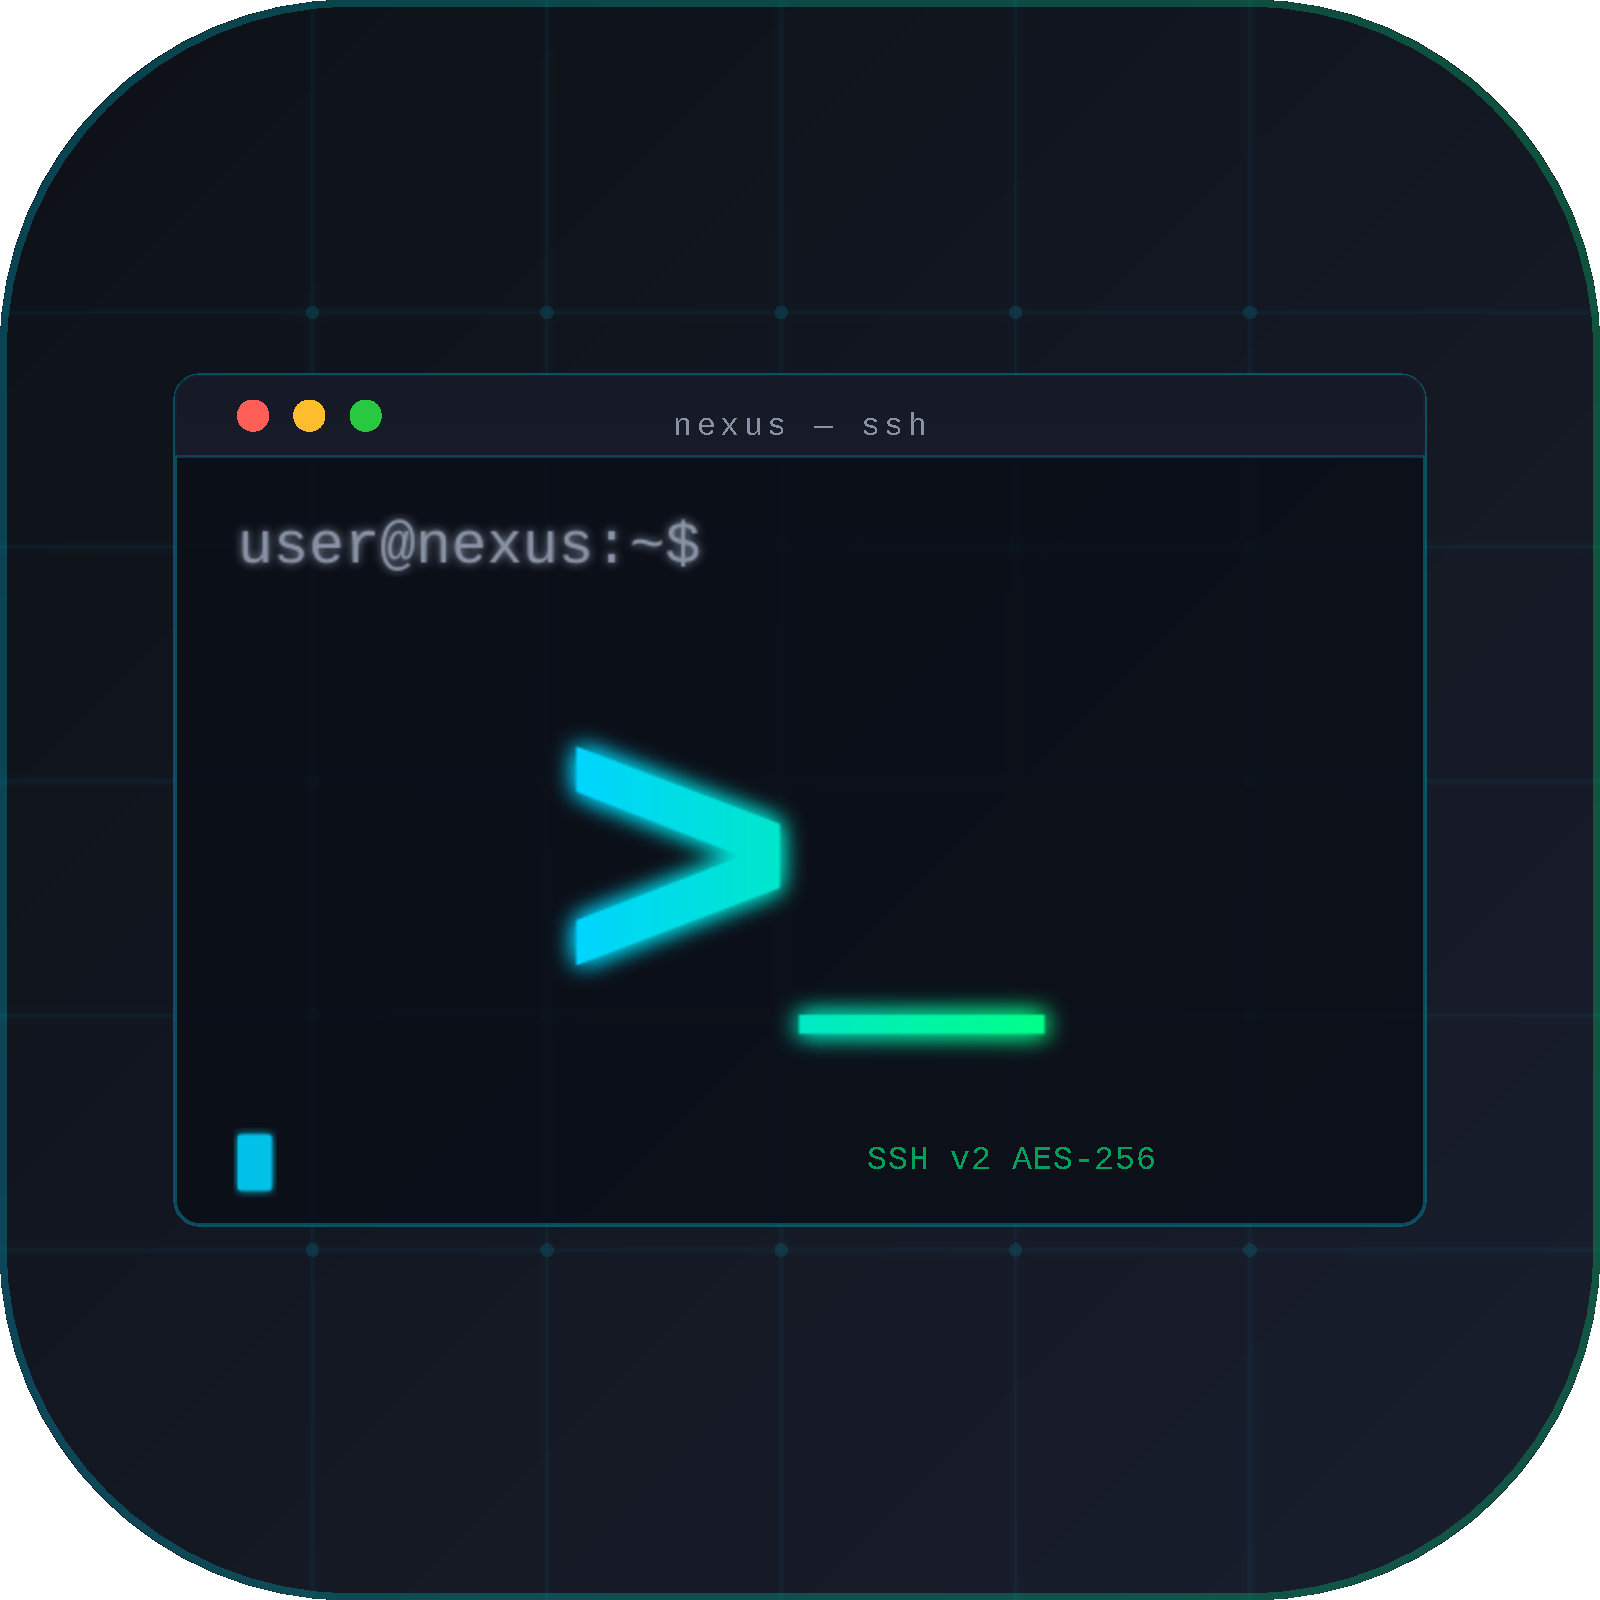
\includegraphics[width=16mm]{img/logo.pdf}\par\vspace{6pt}
{\heavy\color{ink}That's the lot.}\par
{\small\color{muted}Go and connect to something. \iRocket}
\end{center}

\end{document}
